\documentclass{polytech/polytech}
\usepackage{dirtree}
% zone du préambule
\typereport{ppgldi4}

\reportyear{2017-2018}

\title{Création de fond de planning}
% https://gitlab.projectsforge.org/polytech/polytech/wikis/home

\student{Hanyuan}{Peng}{hanyuan.peng@etu.univ-tours.fr}
\student{Stéphane}{Deluce}{stephane.deluce@etu.univ-tours.fr}

\academicsupervisor[di]{Christophe}{Lenté}{christophe.lente@univ-tours.fr}

\resume{Le programme devra créer un fond de planning en Excel afin de faciliter la création des emplois	du temps. Grossièrement, le fond de de planning se présente comme un quadrillage avec en ligne les cours (CM, TD, TP) et en colonne les semaines. Des formules de calculs sont ajoutées à certaines cases afin de comptabiliser les heures placées. Le programme prendra en entrée un fichier excel (ou au pire csv) contenant une maquette et les enseignants affectés. Il fournira en sortie un fichier excel.}
\motcle{Java}
\motcle{Excel}
\motcle{Apache POI}

\abstract{The program will need to create an Excel planning fund to facilitate the creation of timetables. Roughly speaking, the planning background is presented as a grid with on-line courses (CM, TD, TP) and in columns during the weeks. Calculation formulas are added to certain boxes in order to count the hours placed. The program will take an excel (or at worst csv) file containing a mock-up and the affected teachers as input. It will output an excel file.}
\keyword{Java}
\keyword{Excel}
\keyword{Apache POI}


% zone du préambule
\begin{document}
	% zone du contenu du document
	\chapter{Introduction}
	\section{Présentation du projet}
	L’objectif de projet est de développer un programme qui devra créer un fond de planning en Excel afin de faciliter la création des emplois du temps.
	Grossièrement, le fond de de planning se présente comme un quadrillage avec en ligne les cours (CM, TD, TP) et en colonne les semaines.
	Des formules de calculs sont ajoutées à certaines cases afin de comptabiliser les heures placées.
	Il est utilisé pour répartir les heures de CM, TD, TP par semestres et par enseignants.

	Le programme prendra en entrée un fichier excel contenant une maquette et les enseignants affectés. Il fournira en sortie un fichier excel.
	Il sera possible d'ajouter un fichier d'entrée pour les éléments manquants, comme les dates rentrées, de vacances ...

	\chapter{Environnement de développement}
	\section{Langage de programmation}

	Java nous à été imposé comme langage de programmation.
	Nous avons choisi comme IDE \href{http://www.eclipse.org}{Eclipse} pour développer le programme, car c'est un outil que nous avions tous les deux déjà utilisé.

	%\pagebreak

	\section{Outils de gestion de projet}

	Nous avons fais le choix d'utiliser \href{https://trello.com/}{Trello} afin de gérer les tâches de notre projet.
	Trello est un \textit{Kanban} en ligne, il nous permet de visualiser les taches qu'il nous reste à faire ainsi que les taches sur lesquelles travail notre binôme.

	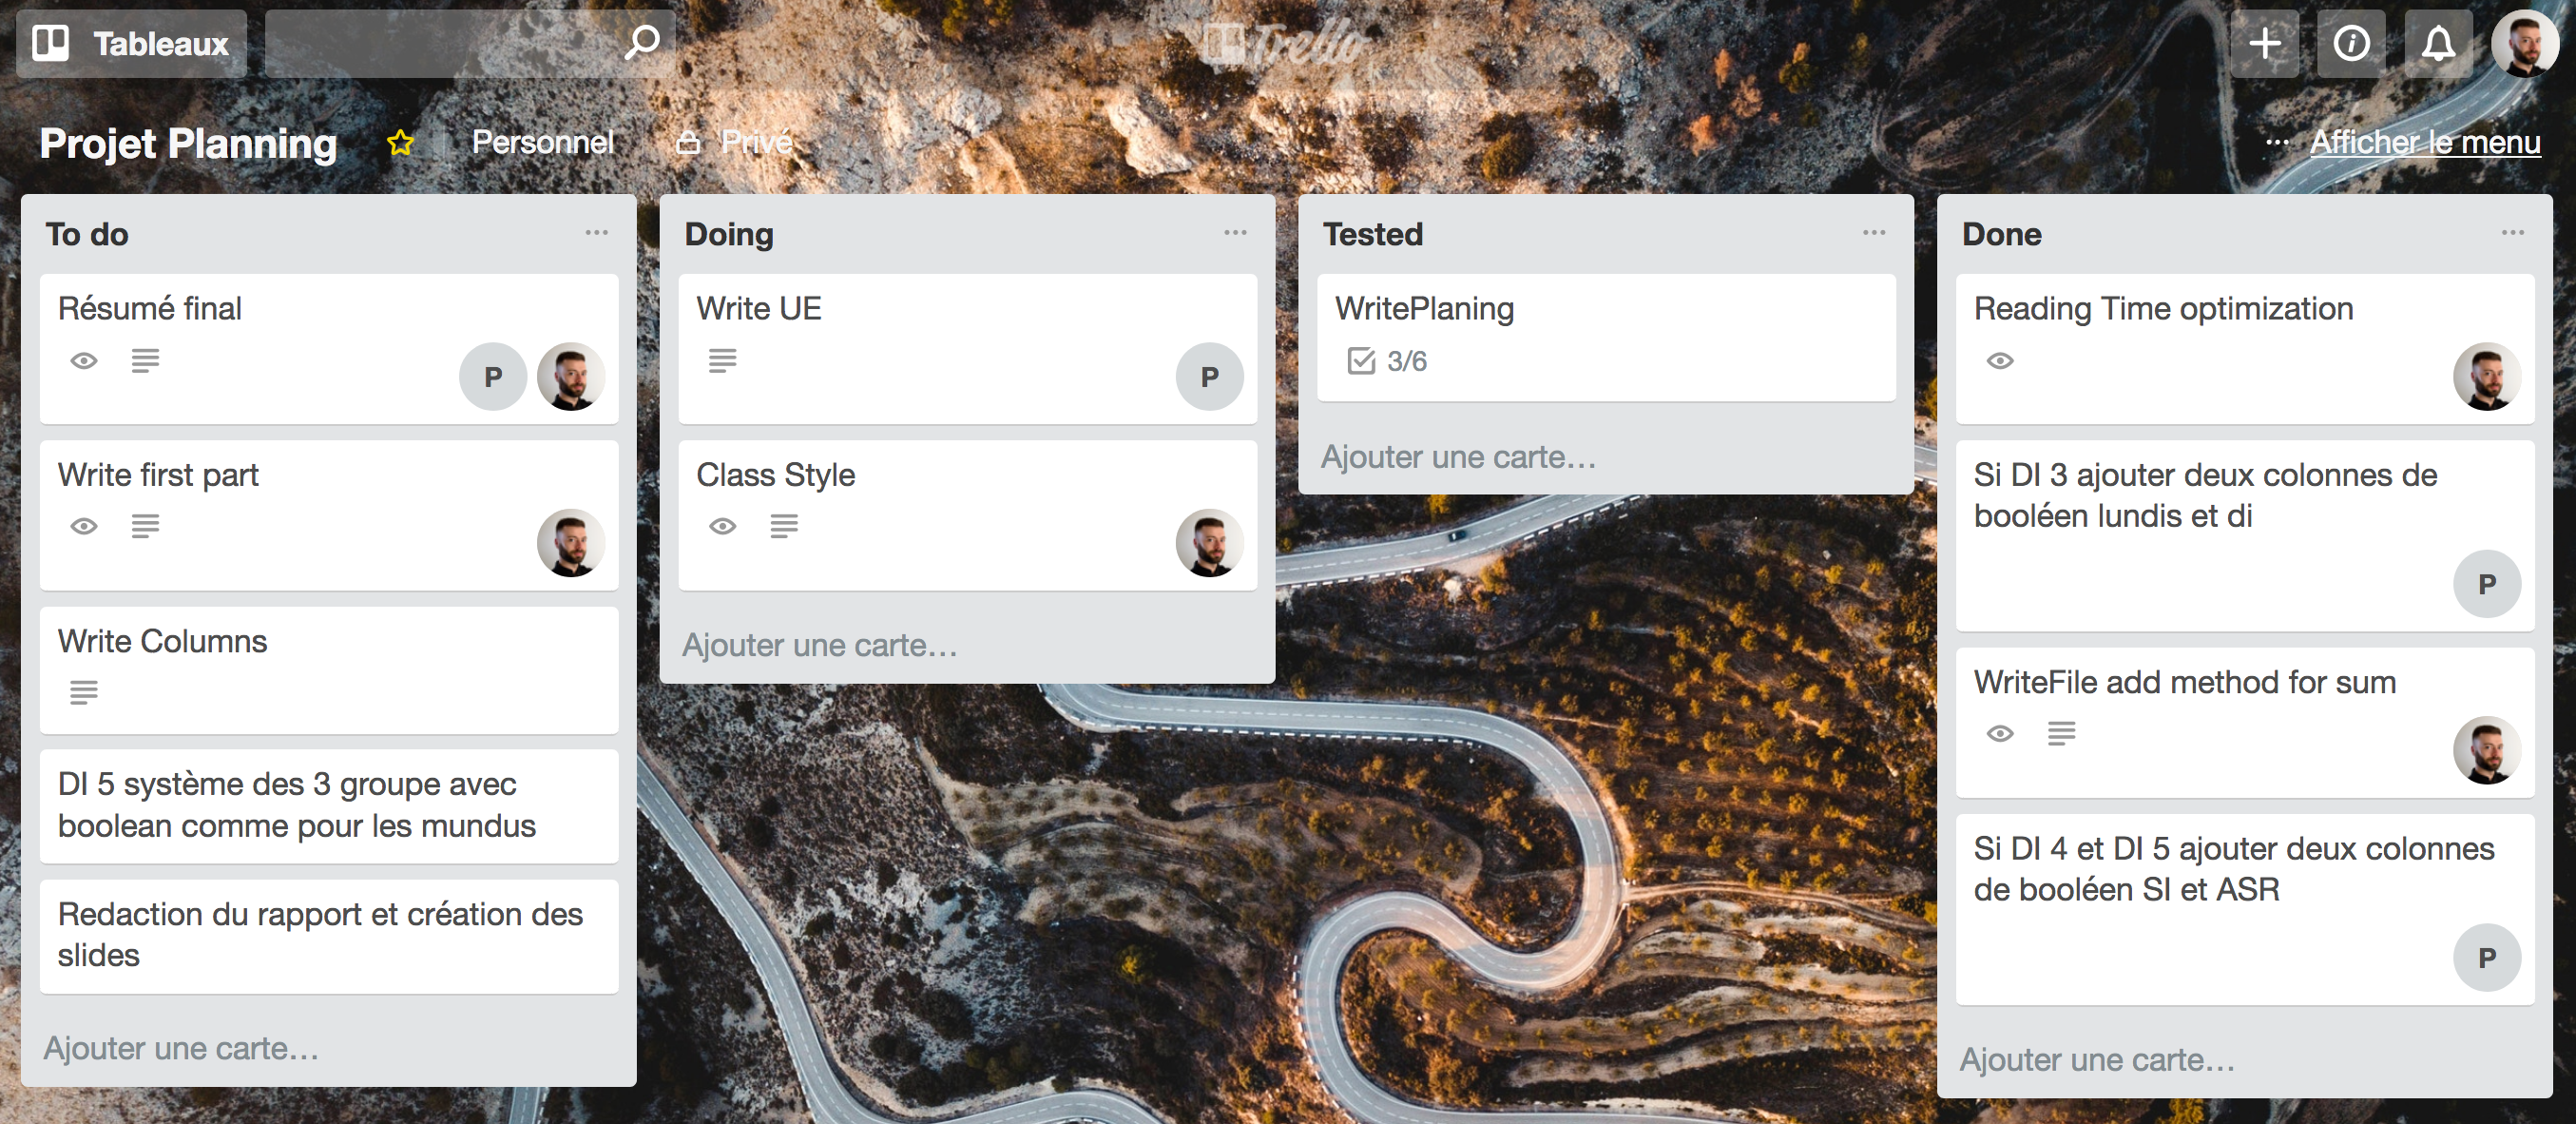
\includegraphics[width=\textwidth]{./img/trello.png}

	Nous avons mis en place un \href{https://git-scm.com/}{Git} comme système de versionning, et nous avons fais le choix d'heberger notre code à l'aide de GitLab qui nous permet de faire des projets privés.
	\href{https://about.gitlab.com/}{GitLab} nous permettais aussi de centraliser notre code à un même endroit.

	Notre projet utilisera des bibliothèques, pour simplifier la gestion des dépendances, nous avons fait le choix d'utiliser \href{https://maven.apache.org/}{Maven} qui est un gestionnaire de dépendances pour Java.

	\chapter{Étude de projet}
	\section{Analyse des besoins}

	Le logiciel que nous allons développer devra être capable de générer un ou plusieurs fond de planning.

	Il devra être capable de lire des fichiers Excel de type Xlsx,
	mais aussi pouvoir créer des fichier Excel de même type, avec des formules, de la mise en forme et de la mise en forme conditionnelle.

	\section{Spécifications Fonctionnelles}

	Le logiciel que nous allons développer aura comme fonction de générer un ou plusieurs fond de planning. Pour effectuer cette tâche, il devra en remplir plusieurs autres.

	\begin{enumerate}
		\item \textbf{Lire un fichier Excel}
		\begin{enumerate}
			\item Rôle :  Primaire
			\item Spécification :
			\begin{itemize}
				\item[-] Entrée : Fichier Excel
				\item[-] Sortie : Données lues
				\item[-] Pré-condition : Fichier Excel au format valide
				\item[-] Post-condition :
				\begin{itemize}[label=\textbullet, font=\LARGE]
					\item Cette fonction a pour but récupérer les données utiles à la génération d'un fond de planning, contenue dans un fichier Excel.
				\end{itemize}
			\end{itemize}
		\end{enumerate}

		\item \textbf{Parser les données récupérés dans les fichiers Excel}
		\begin{enumerate}
			\item Rôle :  Primaire
			\item Spécification :
			\begin{itemize}
				\item[-] Entrée : Données brutes
				\item[-] Sortie : Données structurées
				\item[-] Pré-condition : Les données brutes doivent être valides
				\item[-] Post-condition :
				\begin{itemize}[label=\textbullet, font=\LARGE]
					\item Cette fonction a pour but structurer les données bruts.
				\end{itemize}
			\end{itemize}
		\end{enumerate}

		\item \textbf{Stocker les données}
		\begin{enumerate}
			\item Rôle :  Primaire
			\item Spécification :
			\begin{itemize}
				\item[-] Entrée : Données structurées
				\item[-] Sortie : Objets construis avec les données
				\item[-] Pré-condition : Les données brutes doivent être valides
				\item[-] Post-condition :
				\begin{itemize}[label=\textbullet, font=\LARGE]
					\item Cette fonction sera utile pour stocker les données structurées dans des objets
				\end{itemize}
			\end{itemize}
		\end{enumerate}

		\item \textbf{Générer un objet Planning}
		\begin{enumerate}
			\item Rôle :  Primaire
			\item Spécification :
			\begin{itemize}
				\item[-] Entrée : Objets construis avec les données
				\item[-] Sortie : Objets planning
				\item[-] Pré-condition : Tous les objets doivent être présents
				\item[-] Post-condition :
				\begin{itemize}[label=\textbullet, font=\LARGE]
					\item Cette fonction a pour un objet fond de planning complet.
				\end{itemize}
			\end{itemize}
		\end{enumerate}

		\item \textbf{Créer un fichier Excel contenant le fond de planning}
		\begin{enumerate}
			\item Rôle :  Primaire
			\item Spécification :
			\begin{itemize}
				\item[-] Entrée : Objets planning
				\item[-] Sortie : Fichier Excel
				\item[-] Pré-condition : L'objet doit être valide
				\item[-] Post-condition :
				\begin{itemize}[label=\textbullet, font=\LARGE]
					\item Cette fonction a pour but transformer un objet planning en un fichier Excel.
				\end{itemize}
			\end{itemize}
		\end{enumerate}
	\end{enumerate}

	\pagebreak

	\section{Modélisation}

	Nous avons fais le choix d'utiliser l'architecture MVC (Modèle-vue-contrôleur) pour notre projet.
	La partie contrôleur est utilisée pour lire les données d'entrée, analyser les donnée et générer le planning.
	La partie modèle est utilisée pour stoker les données qu'on a lit et qu'on utilisera pour le planning.
	La partie vue est utilisée pour permettre les utilisateurs saisissent les commandes pour la génération des fond de planning.

	\subsection{UML}
	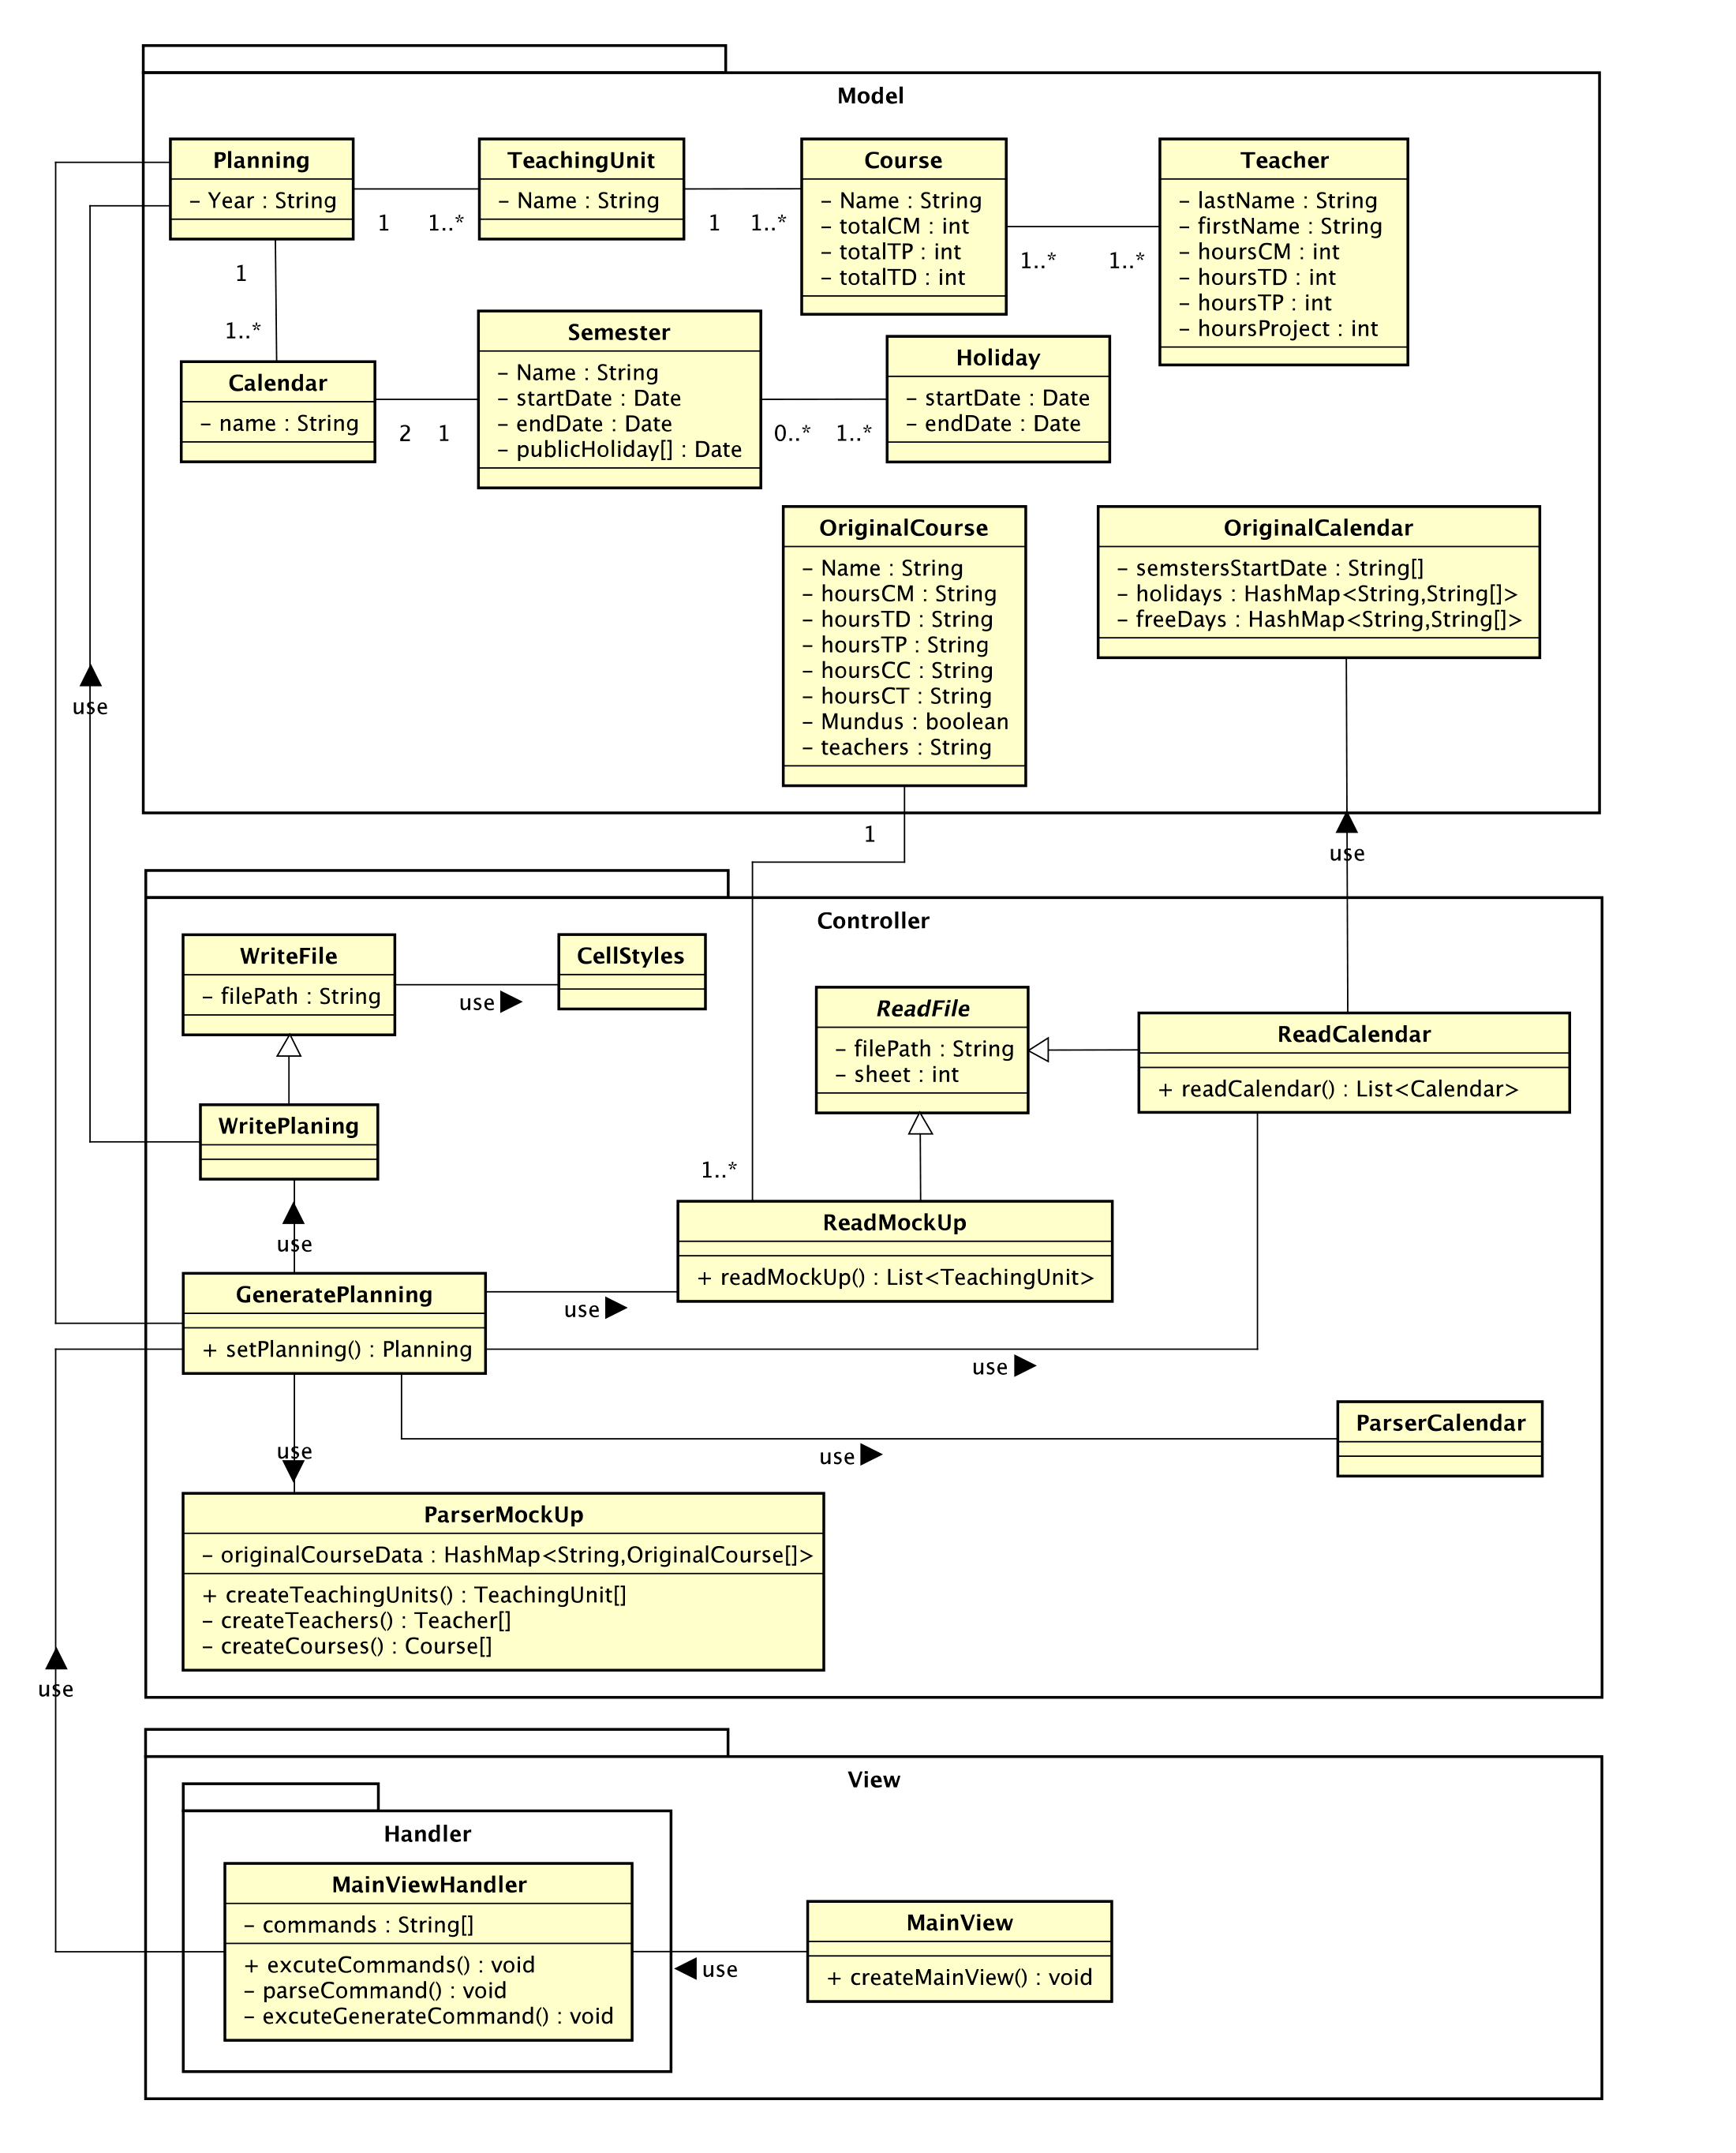
\includegraphics[scale=0.2]{./img/Diagram.png}

	\pagebreak

	\subsection{Définitions des classes}
	\subsubsection{Modèle}
		\begin{enumerate}
			\item \paragraph{class Calendar}

			Le but de cette classe est de stocker les informations d'un calendrier. Un calendrier représente deux semestres.

			\textbf{Attributs :}
				\begin{itemize}
					\item[-] Le nom de calendrier, il stocke le nom de l'année.
					\item[-] La liste des semestres, une arrayList des semestres de l'année.
				\end{itemize}

			\item \paragraph{class OriginalCalendar}

			Le but de cette classe est de stocker les informations originaux qui sont lues à partir de fichier calendrier pour analyser.

			\textbf{Attributs :}
				\begin{itemize}
					\item[-] Un LinkedHashMap des semestres, il stocke les informations originaux des semestres.
					\item[-] Un LinkedHashMap des vacances, il stocke les informations originaux des vacances d'une année.
					\item[-] Un LinkedHashMap des jours libres, il stocke les informations originaux des jours libres d'une année.
				\end{itemize}

			\item \paragraph{class Teacher}

			Le but de cette classe est de stocker les informations des professeurs d'un cours.

			\textbf{Attributs :}
				\begin{itemize}
					\item[-] Le nom de professeur.
					\item[-] L'heure totale de CM que ce professeur fera.
					\item[-] L'heure totale de TD que ce professeur fera.
					\item[-] L'heure totale de TP que ce professeur fera.
					\item[-] L'heure totale de Projet que ce professeur fera.
					\item[-] L'heure totale de TD pour Mundus que ce professeur fera.
					\item[-] L'heure totale de TP pour Mundus que ce professeur fera.
				\end{itemize}

			\item \paragraph{class Course}

			Le but de cette classe est de stocker les informations de cours.
			\textbf{Attributs :}
				\begin{itemize}
					\item[-] Le nom de cours;
					\item[-] Une liste de tous les professeurs qui font ce cours.
					\item[-] L'heure totale de CM de ce cours.
					\item[-] L'heure totale de TD de ce cours.
					\item[-] L'heure totale de TP de ce cours.
					\item[-] L'heure totale de Projet de ce cours.
					\item[-] Un booléen pour marquer si ce cours a un cc.
					\item[-] Un booléen pour marquer si ce cours a un ct.
					\item[-] Un booléen pour marquer si ce cours est un cours de type Mundus.
					\item[-] Un string pour noter le type de ce cours est SI ou ASR.
				\end{itemize}
			\pagebreak

			\item \paragraph{class OriginalCourse}

			Le but de cette classe est de stocker les informations originaux qui sont lues à partir de fichier maquette pour analyser.

			\textbf{Attributs :}
				\begin{itemize}
					\item[-] Le nom de cours;
					\item[-] Une chaîne de caractère de l'affectation de professeurs.
					\item[-] L'heure totale de CM de ce cours.
					\item[-] L'heure totale de TD de ce cours.
					\item[-] L'heure totale de TP de ce cours.
					\item[-] L'heure totale de Projet de ce cours.
					\item[-] Un booléen pour marquer si ce cours a un cc.
					\item[-] Un booléen pour marquer si ce cours a un ct.
					\item[-] Un booléen pour marquer si ce cours est un cours de type Mundus.
				\end{itemize}

			\item \paragraph{class TeachingUnit}

			Le but de cette classe est de stocker les informations d'une unité d'enseignement (UE).

			\textbf{Attributs :}
				\begin{itemize}
					\item[-] Le nom de UE;
					\item[-] Une liste de cours de cette UE.
				\end{itemize}

			\item \paragraph{class FreeDay}

			Le but de cette classe est de stocker les informations d'un jour libre.

			\textbf{Attributs :}
				\begin{itemize}
					\item[-] Le nom de ce jour libre.
					\item[-] La date de ce jour.
					\item[-] Le nombre de créneaux
				\end{itemize}

			\item \paragraph{class Planning}

			Le but de cette classe est de stocker les informations d'un planning pour l'éciture.

			\textbf{Attributs :}
				\begin{itemize}
					\item[-] L'année du planning que on veut générer.
					\item[-] Une liste de l'unité enseignement de cette année dans un planning.
					\item[-] Un calendrier de cette année.
				\end{itemize}

			\item \paragraph{class Holiday}

			Le but de cette classe est de stocker les informations des vacances.

			\textbf{Attributs :}
				\begin{itemize}
					\item[-] Le nom des vacances.
					\item[-] La date début des vacances.
					\item[-] La date fin des vacances.
				\end{itemize}

			\item \paragraph{class Semester}

			Le but de cette classe est de stocker les informations d'une semestre.

			\textbf{Attributs :}
				\begin{itemize}
					\item[-] Le nom d'une semestre, par exemple " S5 ".
					\item[-] La date début d'une semestre.
					\item[-] La date fin d'une semestre.
					\item[-] Une liste de jour libre.
					\item[-] Une liste des vacances.
				\end{itemize}
		\end{enumerate}
		\pagebreak
	\subsubsection{Contrôleur}
		\begin{enumerate}
			\item \paragraph{class GeneratePlanning}
			Le but de cette classe est de générer le planning à partir des informations stockées dans les objets Planning.

			\item \paragraph{class ReadFile}
			Le but de cette classe est de fournir les fonctions basiques pour lire le fichier maquette et le fichier calendrier.

			\item \paragraph{class WriteFile}
			Le but de cette classe est de fournir les fonctions basiques pour écrire le planning dans un fichier Excel.

			\item \paragraph{class ParserCalendar}
			Le but de cette classe est d'analyser les informations de calendrier à partir d'un objet OriginalCalendar.
			\item \paragraph{class ReadMockUp}
			Le but de cette classe est de lire le fichier maquette et de stocker les informations originaux d'un cours dans un objet OriginalCourse. On utilise la méthode getTeachingUnits de cette classe pour retourner un LinkedHashMap des unités d'enseignement. On utilisera ce LinkedHashMap pour analyser les informations d'une UE.
			\item \paragraph{class WritePlanning}
			Le but de cette classe est d'écrire les informations d'un objet planning dans un fichier Excel.
			\item \paragraph{class ParserMockUp}
			Le but de cette classe est d'analyser les informations de maquette à partir du . LinkedHashMap qui est fourni par la classe ReadMockUp.
			\item \paragraph{class StylesLib}
			Le but de cette classe est de fournir des style de cellule.
			\item \paragraph{class ReadCalendar}
			Le but de cette classe est de lire le fichier calendrier et de stocker les informations originaux d'un calendrier dans un objet OriginalCalendar.
			\item \paragraph{class ToolBox}
			Le but de cette classe est de fournir des méthodes comme vérifier le type de cours.
		\end{enumerate}

	\subsubsection{Vue}
	\begin{enumerate}
		\item \paragraph{class Mainview}
		Le but de cette classe est de créer une vue pour l'utilisateur.

		\item \paragraph{class MainViewHandler}
		Le but de cette classe est de traiter les commandes qui est saisies par l'utilisateur et de faire l'exécution des commandes en appelant aux contrôleurs.
	\end{enumerate}
	\chapter{Planification}

	\section{Diagramme de Gantt}

	Pour mener à terme ce projet, il nous a fallu le décomposer en taches, leurs déterminer une priorité et en estimer leurs durées. Ces informations nous ont permis de réaliser un diagramme de Gantt prévisionnel qui à été mis a jour en cours de projet.

	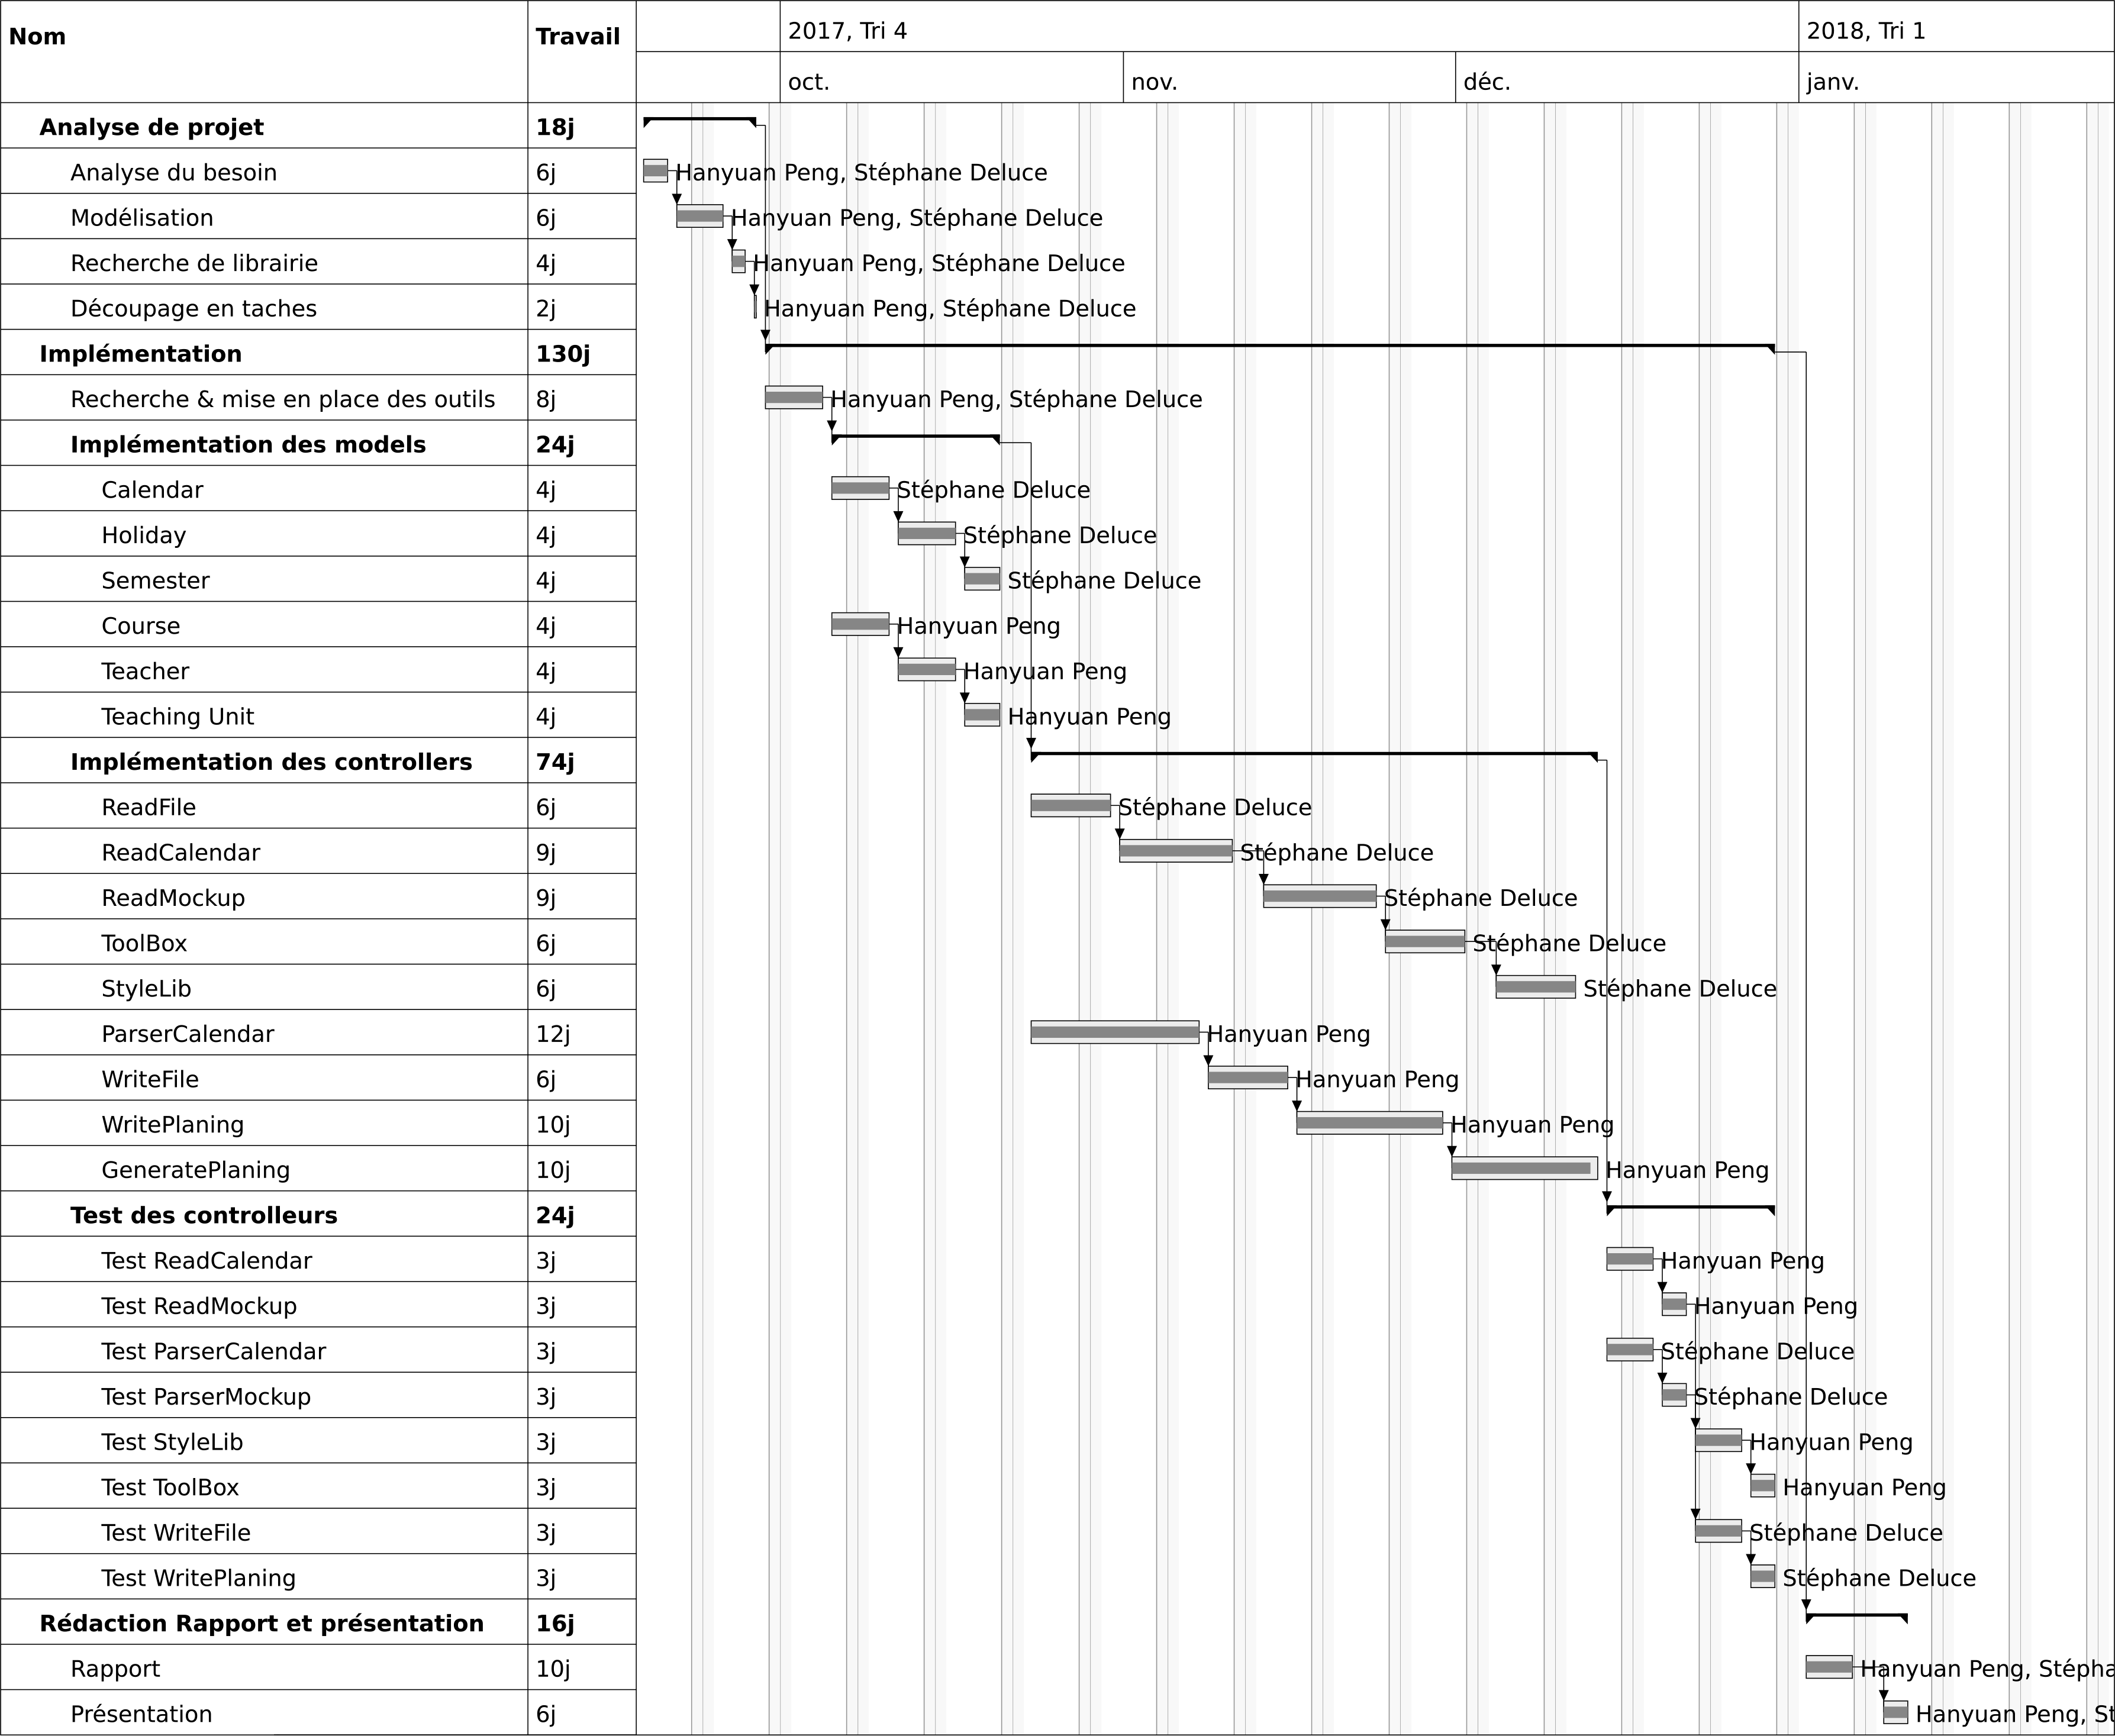
\includegraphics[width=\textwidth]{./img/Gantt.png}

	Nous avons paramétré le calendrier avec deux heures de travail par jour, avec des semaines de 5 jours.
	La répartition de notre travail n'as pas forcément respecté ce calendrier, mais la quantité de travail fournie est équivalente.

	\section{Répartition des tâches}
	+++++++++++++++++++++++++++++++++++++++++++++

	Nous avons choisi de se diviser le travail par classes.
	Avec des points régulier pour expliquer l'avancé de notre travail, et partager nos remarques et
	interrogations

	+++++++++++++++++++++++++++++++++++++++++++++

	\chapter{Implémentation}

	+++++++++++++++++++++++++++++++++++++++++++++

	\section{Choix de bibliothèques}

	Pour réaliser la lecture et l'écriture des fichiers Excel, nous avons fais le choix d'utiliser une bibliothèque.
	Après avoir effectué des recherches, nous avons trouvés deux bibliothèques qui pourraient répondre à nos besoins.

	Le première, \href{http://jexcelapi.sourceforge.net/}{Java Excel API}, qui est un projet Open Source mis à jour pour la dernière fois en 2009.

	\label{lib}
	La seconde, \href{http://poi.apache.org}{POI Apache}, gratuit, mais sous licence \href{https://www.apache.org/licenses/}{Apache}.
	Elle à été mise a jour pour la dernière fois le 15 Septembre 2017.
	Ce n'est pas forcement gage de bonne qualité, mais ça signifie que le projet évolue et qu'il n'est pas à l'abandon.
	Cette bibliothèque est très bien documenté, et utilisé par une large communauté.

	Après quelques essais avec les deux bibliothèques, nous avons fais le choix d'utiliser \textbf{POI Apache} pour réaliser ce projet.

	\section{Organisation}

	%Nous utilisons Maven pour la gestion de bibliothèque.
	Comme vu précédemment (\ref{lib}), nous avons choisis \textbf{POI Apache} comme bibliothèque pour la lecture / écriture de fichiers Excel.
	Pour l'ajouter à notre projet, il faut ajouter ces lignes à notre fichier pom.xml.
	Maven récupèrera automatiquement les bibliothèques renseignées dans ce fichier.

	\begin{latexsource}
	<dependency>
		<groupId>org.apache.poi</groupId>
		<artifactId>poi-ooxml</artifactId>
		<version>3.17</version>
	</dependency>
	\end{latexsource}

	\subsection{Organisation des fichiers}
	+++++++++++++++++++++++++++++++++++++++++++++

	Nous avons commencé par développer les modèles, puis les contrôleurs pour finir avec la vue.

	+++++++++++++++++++++++++++++++++++++++++++++


	Les groupes des classes modèles, vues et contrôleurs ont chacunes été placés dans un package, ce nous donne l'arborescence suivante :

	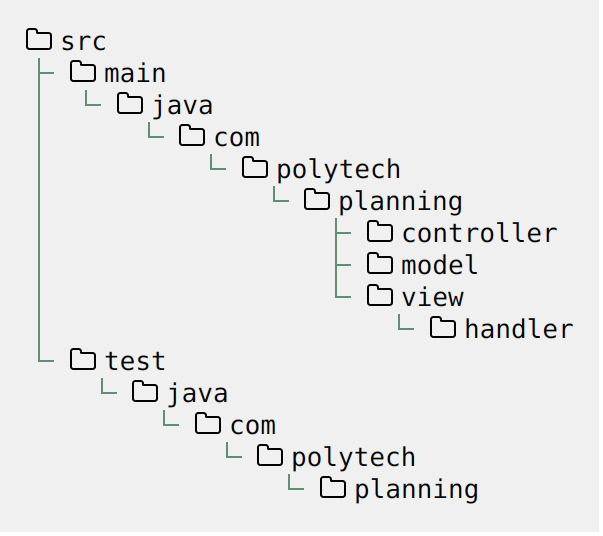
\includegraphics[width=\textwidth]{./img/folder-planning.png}

	\section{Tests et validation}

	Les tests unitaires ont été réalisés après l'écriture des méthodes de chaque classes.
	Ils ont été fais de manières croisées, les méthodes écrites par l'un de nous deux ont été testés par l'autre.
	Nous avons utilisé la bibliothèque \textbf{JUnit} pour réaliser nos tests unitaires.

	Certains tests visuels, pour le formatage des feuilles Excel sont faites visuellement.
	Nous n'avons pa trouvé d'autres méthodes pour vérifier ceci.

	\subsection{Résultat d'exécution}
	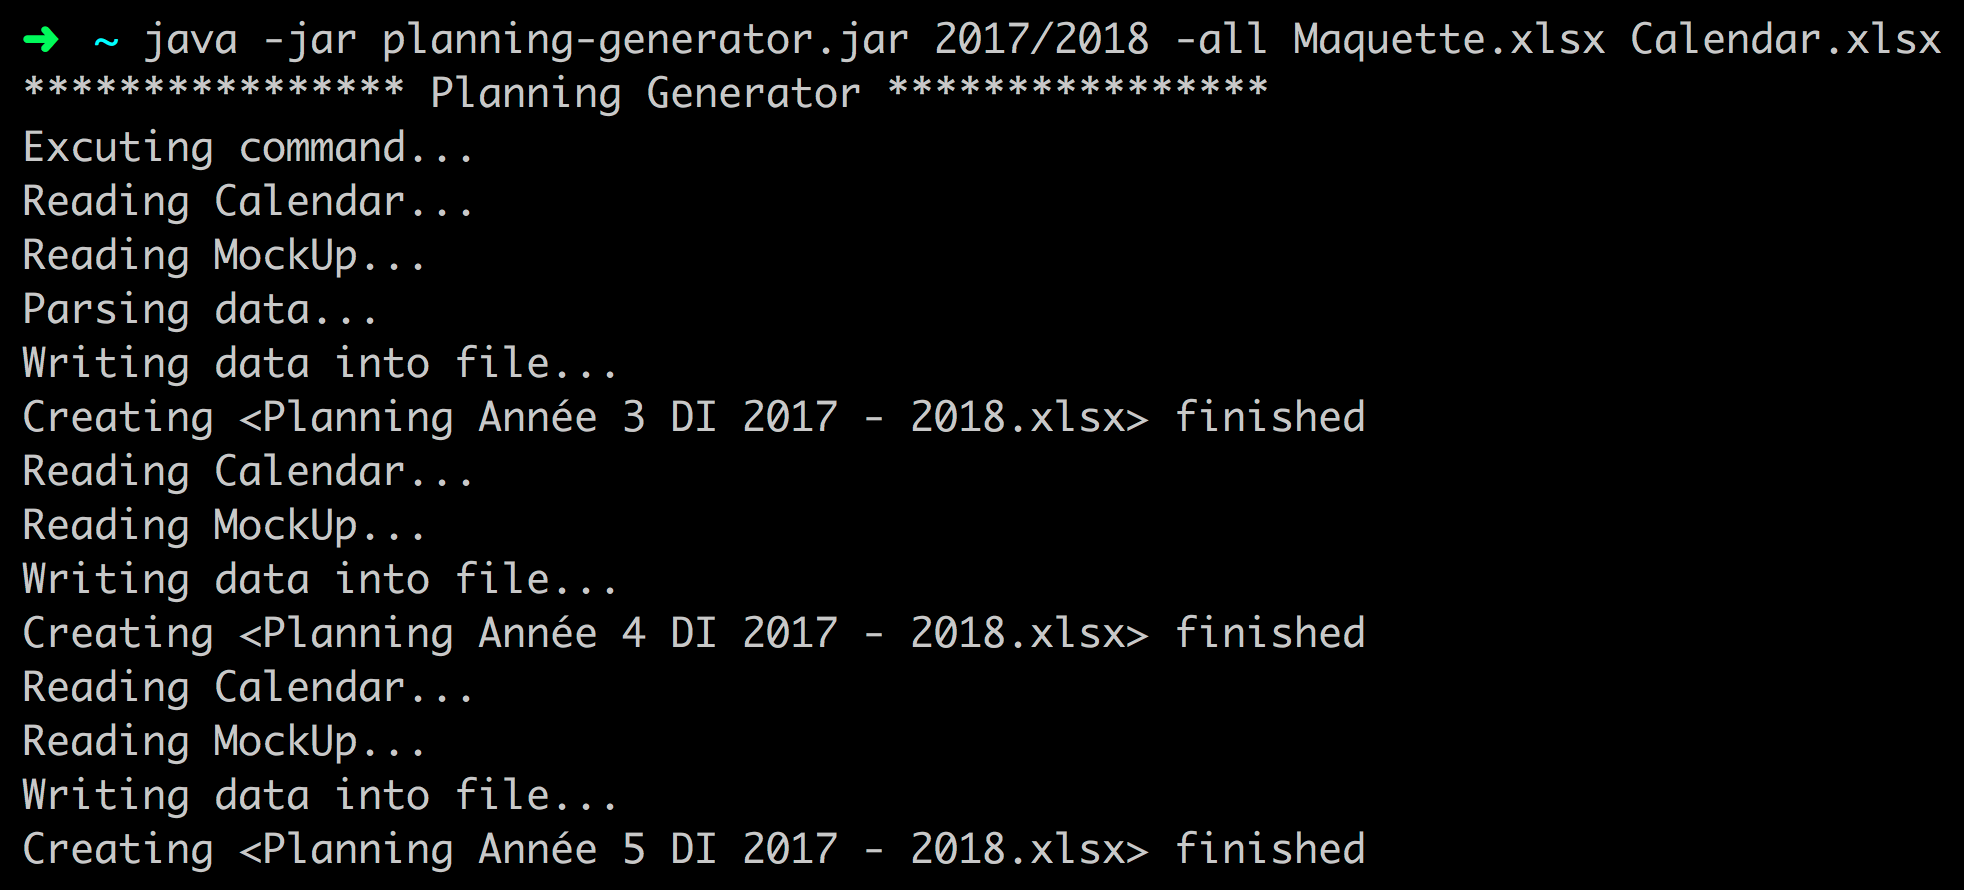
\includegraphics[width=\textwidth]{./img/excution_result2.png}

	\section{Documentation}
	+++++++++++++++++++++++++++++++++++++++++++++

	Classes documentés (JavaDoc) pour évolutivité, ...

	+++++++++++++++++++++++++++++++++++++++++++++
	\chapter{Annexes}

	\section{Manuel d'utilisation}
	Comme nous n'avions rien d'imposé pour la création du manuel utilisateur, nous avons fais le choix d'utiliser AsciiDoc.

	
\includepdf[pages=3-, offset=0 0]{../manuel.pdf}
\end{document}
